\documentclass{ctexart}

% Language setting
% Replace `english' with e.g. `spanish' to change the document language
\usepackage{xeCJK}
\usepackage{subfigure}

% Set page size and margins
% Replace `letterpaper' with `a4paper' for UK/EU standard size
\usepackage[letterpaper,top=2cm,bottom=2cm,left=3cm,right=3cm,marginparwidth=1.75cm]{geometry}

% Useful packages
\usepackage{amsmath}
\usepackage{graphicx}
\usepackage[colorlinks=true, allcolors=blue]{hyperref}

\title{项目报告}
\author{王歆玥,杨泰格,朱震阳}

\begin{document}
\maketitle

\section{引言}

本项目为SI100B课程的最终项目,项目文件已上传到\href{https://github.com/yangtaige/O.o}{https://github.com/yangtaige/O.o}。

我们制作了一款Rougelike类型的游戏。玩家初始出生在城市,拥有30金币武装自己,随后可通过传送门进入野外与怪物搏斗。

战斗采用回合制,玩家与怪物轮流攻击,直到一方死亡。游戏中有三种怪物:脆皮神射手骷髅头、血牛刮痧飞天猴、高攻高防精英绿皮人,每种怪物的属性都不一样。
    
玩家击败怪物后可以获得金钱,击败强力的绿皮人可以获得相对更多的金币,玩家每次进入野外时怪物都会变得更强,相应地,玩家击败怪物所能获得的金币也越多。
    
返回城市可以用金币购买升级:商店界面采用鼠标操作,选择自己想购买的升级并点击即可将其收入囊中。商店中还存在着需要献祭自己的生命才能购买的神秘商品,其实际作用为削弱怪物的等级,但你仍然可以从怪物身上获取相当于未购买神秘物品时怪物等级所对应的金币。
    
击败Boss大扑棱蛾子就能游戏通关,并显示通关时长。

\section{项目实施}

\subsection{场景}
\subsubsection{场景数量}
我们的游戏中一共有三个场景:

1、城市:玩家可以在此处与NPC对话,在商店中用金钱进行交易,见图\ref{fig:场景1};

2、野外:玩家可以在此处与怪物战斗获取金钱,见图\ref{fig:场景2};

3、Boss房:玩家进入Boss房后只能与Boss决一死战,见图\ref{fig:场景3}。

我们的场景由地图砖块与障碍物构成,在每一帧中,程序会一个一个地渲染地图砖块,拼接起来的砖块形成了一个完整的场景。
\begin{figure}
\centering
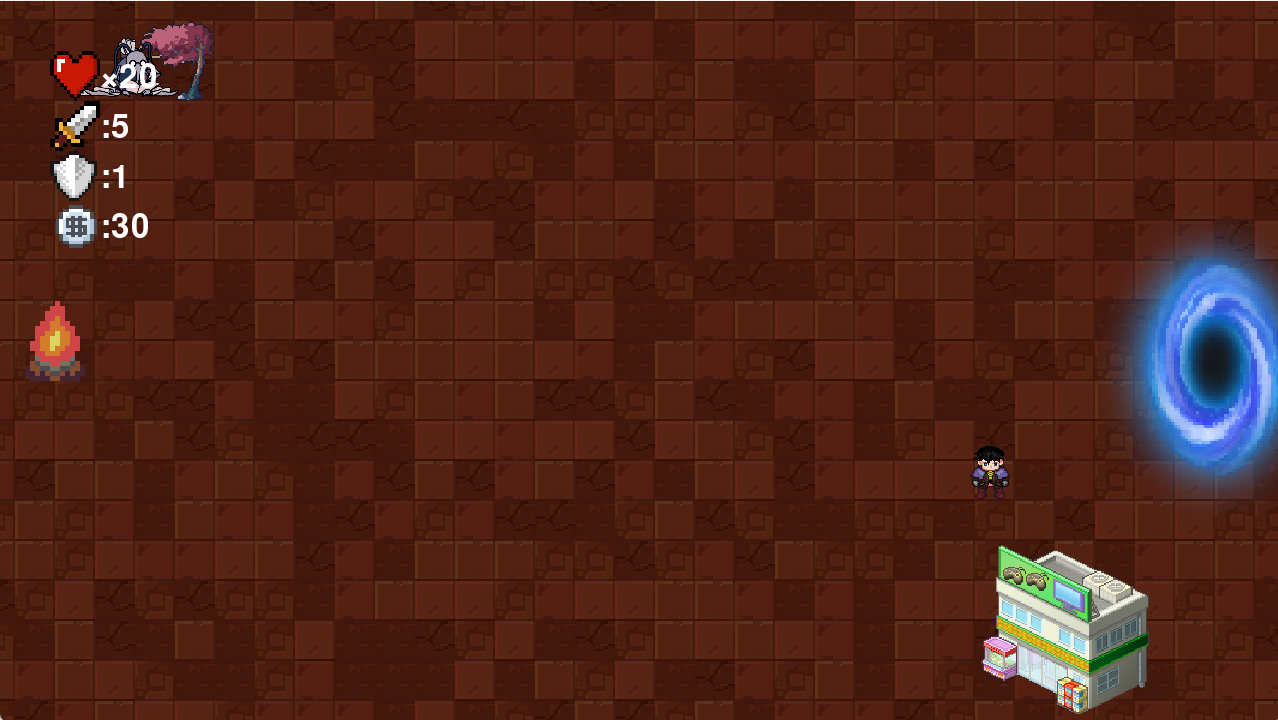
\includegraphics[width=0.7\linewidth]{场景1.png}
\caption{\label{fig:场景1}城市场景}
\end{figure}

\begin{figure}
\centering
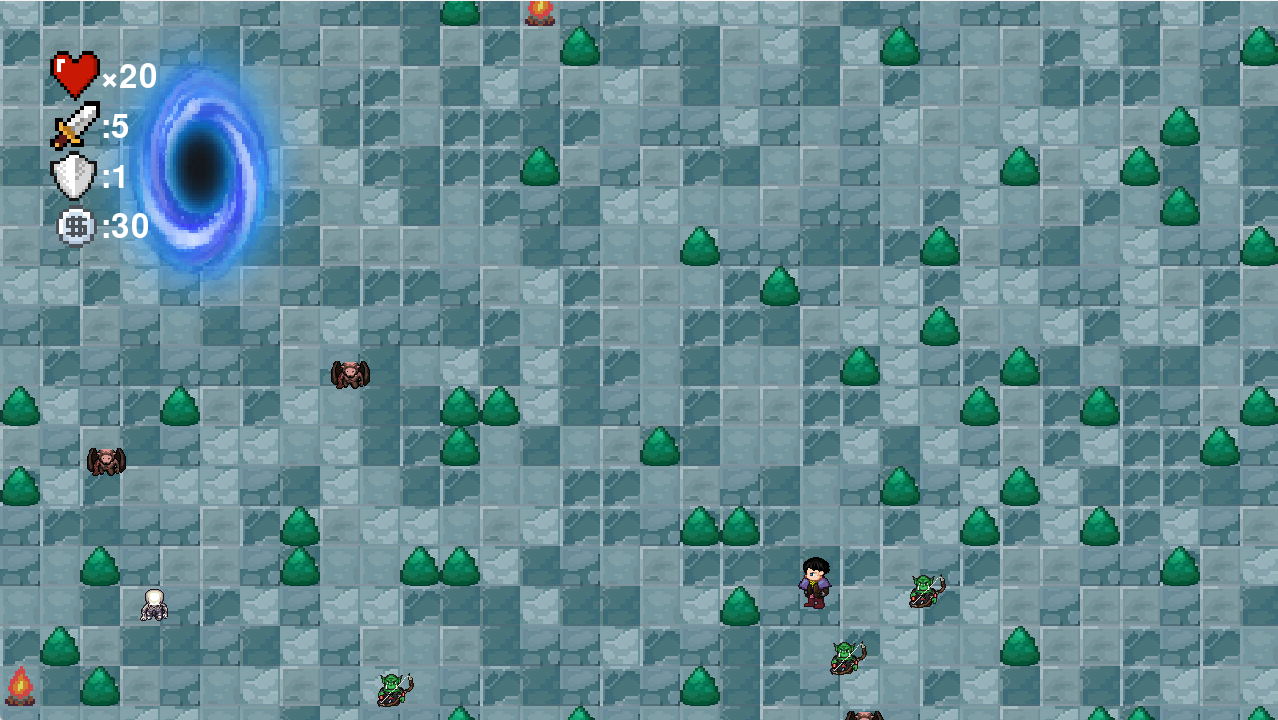
\includegraphics[width=0.7\linewidth]{场景2.png}
\caption{\label{fig:场景2}野外场景}
\end{figure}

\begin{figure}
\centering
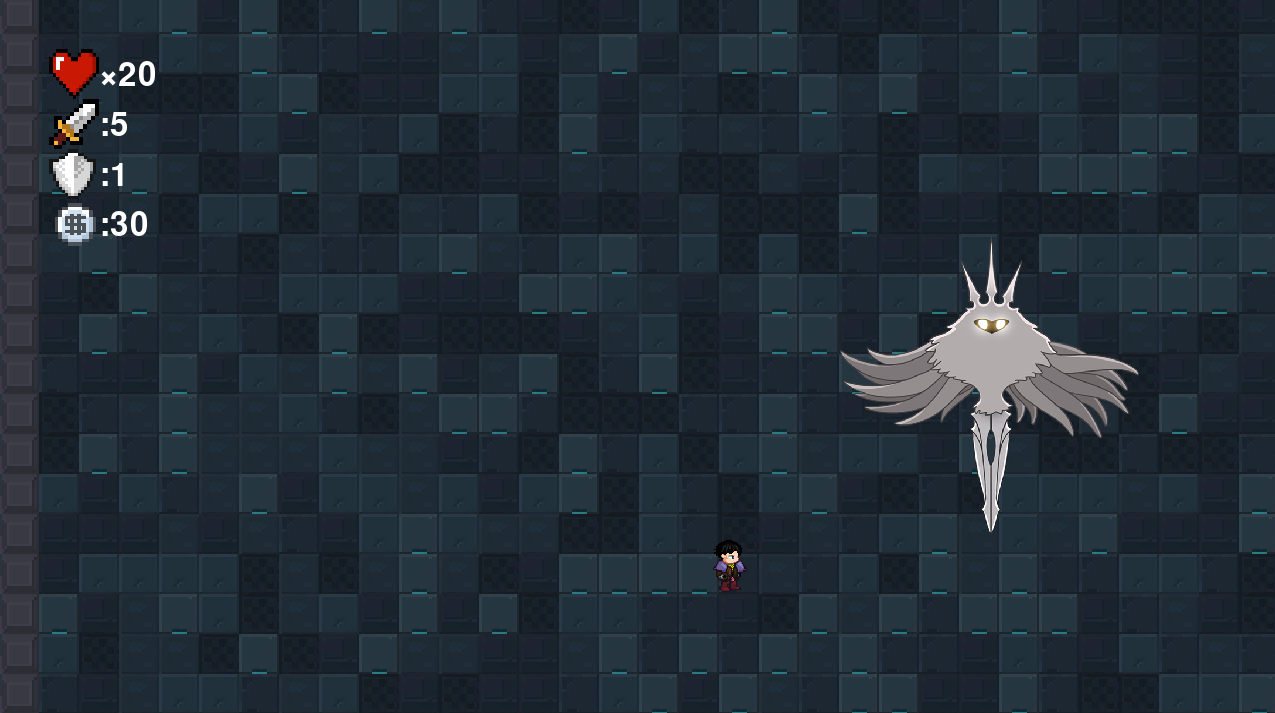
\includegraphics[width=0.7\linewidth]{场景3.png}
\caption{\label{fig:场景3}Boss房场景}
\end{figure}

\subsubsection{大型场景}
我们游戏中的每个场景都是大型场景,都有着可以跟随玩家移动而进行视角移动的摄像头。

镜头移动的原理:每当满足镜头移动的条件时, 所有物体(含地砖、NPC、玩家)都会获得一个偏移量,该偏移量等于在这一帧玩家试图移动的距离,在渲染时所有物体的位置都会加上这个偏移量的相反数。因此,玩家移动了$\left ( \mathrm{d}x,\mathrm{d}y \right ) +  \left ( -\mathrm{d}x,-\mathrm{d}y \right )= \left ( 0,0 \right )$,即在原地不动,其它物体全部移动偏移量的相反数,达到了镜头移动的效果。 

\subsubsection{互动物品}
我们的游戏中有四种互动物品,分别为树、动画树、墙壁与火堆,如图\ref{fig:互动物品}。
\begin{figure}[h]
\centering
\subfigure[树]{\includegraphics[width=0.2\linewidth]{树.png}}
\subfigure[动画树]{
\includegraphics[width=0.2\linewidth]{动画树.png}}
\subfigure[墙壁]{
\includegraphics[width=0.2\linewidth]{墙壁.png}}
\subfigure[火堆]{
\includegraphics[width=0.2\linewidth]{火堆.png}}
\caption{\label{fig:互动物品}互动物品}
\end{figure}

其中,树、动画树与墙壁均起到障碍物的作用,玩家无法跨越这些障碍物。而火堆无法阻挡玩家走动,但玩家在火堆上走动时会持续受到伤害。这写互动物品会在地图砖块后被渲染,形成它们坐落于地图砖块上的效果。它们起到的作用的实现方法会稍后在游戏机制中提及。

\subsection{角色}
\subsubsection{主要角色}
在我们的游戏中,玩家可以通过wasd四个按键操控主要角色四处移动,通过传送门进入其他场景,通过与其他角色碰撞来触发特殊事件。主要角色的移动通过检测按键按下与抬起这两种事件的方法来实现,当按键被按下,角色就会持续朝指定方向移动,按键抬起后,角色不再朝指定方向移动。

玩家的横向移动与纵向移动被写成了两种方法,在每一帧中,程序会先进行横向移动,判断与障碍物的碰撞,若碰撞则撤回横向移动,再进行纵向移动,判断与障碍物的碰撞,若碰撞则撤回纵向移动。这种分开处理横纵移动的移动处理方式使得玩家在障碍物边缘同时按下两个方向键时不会被卡住。

主要角色行走时会播放行走动画,当玩家按下相应按键后,程序会记录下行走朝向,并以此为依据更改主要角色的图片,使图片与行走方向相匹配,并循环播放一组图片以达到动画的效果。

\subsubsection{友好NPC}
在城市场景中存在着两种友好NPC,一种是对话NPC,还有一种是商店NPC,见图\ref{fig:友好NPC}。
\begin{figure}[h]
\centering
\subfigure[对话NPC]{
\includegraphics[width=0.3\linewidth]{对话npc.png}}
\subfigure[商店NPC]{
\includegraphics[width=0.3\linewidth]{商店npc.png}}
\caption{\label{fig:友好NPC}友好NPC}
\end{figure}

当角色与对话NPC碰撞时,会弹出对话框;而角色与商店NPC碰撞时,会弹出购买界面,购买界面采用鼠标操作的形式选择想购买的升级。

\subsubsection{简单敌人}
野外场景中存在着三种简单敌人:脆皮神射手骷髅头、血牛刮痧飞天猴与高攻高防精英绿皮人。
三种敌人的属性都不一样:骷髅头血量与防御较少,但攻击较高;飞天猴血量防御高,攻击低;绿皮人血量防御与攻击都比较高,见图\ref{fig:简单敌人}。三种敌人被击败时都会有倒地动画。
\begin{figure}[h]
\centering
\subfigure[骷髅头]{
\includegraphics[width=0.3\linewidth]{骷髅头.png}}
\subfigure[飞天猴]{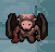
\includegraphics[width=0.3\linewidth]{飞天猴.png}}
\subfigure[绿皮人]{
\includegraphics[width=0.3\linewidth]{绿皮人.png}}
\caption{\label{fig:简单敌人}简单敌人}
\end{figure}

\subsubsection{特殊敌人}
Boss房中存在着一种特殊敌人:大扑棱蛾子,见图\ref{fig:大扑棱蛾子}。击败它就会触发游戏结束事件。
\begin{figure}[h]
\centering
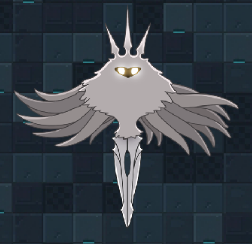
\includegraphics[width=0.7\linewidth]{大扑棱蛾子.png}
\caption{\label{fig:大扑棱蛾子}大扑棱蛾子}
\end{figure}

在我们的程序中,大扑棱蛾子虽然与简单敌人属于两个不同的类,但它们本质上并无不同,微小的区别在于:特殊敌人的属性值很高,没有倒地动画,玩家与其的战斗结束后就会迎来结束界面。

\subsection{游戏机制}
\subsubsection{核心机制}
玩家通过操作主要角色移动来与要互动的角色碰撞,碰撞发生后即会触发相应事件。战斗采用回合制,玩家与怪物交替发起攻击。玩家需要反复击败怪物以获取金钱对自己进行升级,而怪物也会在每次玩家进入野外时变得更强,玩家的最终目标是变得足够强大去挑战Boss大扑棱蛾子。以通关时间作为这次游玩的成绩。

\subsubsection{碰撞系统}
程序通过pygame内置的碰撞检测方法来检测玩家与实体间的碰撞。

当玩家与障碍物发生碰撞时,玩家类中的update方法会撤回玩家在这一帧进行的移动。

当玩家与火堆、NPC、敌人、传送门等实体碰撞时,碰撞检测方法会向事件队列发送相对应的事件,在事件队列中被相继处理。

\subsubsection{资源系统}
玩家击败怪物就可获得金币,怪物的等级越高,玩家获得的金币就越多。金币可以用来在商店中购买升级,提高玩家的战斗力。玩家的血量也是一种资源,玩家需要时刻分配好自己的血量,确保自己不被怪物击杀的同时赚取足够多的金钱再返回城市,商店中也可用血量购买神秘物品怪物削弱。

\subsection{游戏性}
\subsubsection{菜单}
我们的游戏有三种菜单,主菜单、失败界面与胜利界面。

进入游戏与游戏重新开始时会显示主菜单,此时玩家需要按下ENTER键以进入游戏。

当玩家死亡时,会出现失败界面,显示游玩时间,按下ENTER键可重新开始游戏。

当玩家击败大扑棱蛾子时,会出现胜利界面,显示游玩时间,按下ENTER键可重新开始游戏。

\subsubsection{BGM}
我们的游戏在主菜单、失败界面、胜利界面、城市场景、野外场景与Boss房都会播放不同的BGM。

\subsection{代码}
仓库中Game Project为游戏文件。
用编辑器打开Game Project后运行Main.py即可进入游戏。

程序采用面向对象编程的编程方式,代码中难以理解的地方全都添加了注释。

下面罗列程序中的各个文件的相应作用:

    1、Attribute.py
      该文件定义了Collidable类,便于进行实体碰撞后相应事件的触发。

    2、BgmPlayer.py
      该文件负责处理背景音乐的播放。

    3、Gamemanager.py
      该文件定义了GameManager类,该类负责管理游戏。
      玩家、场景、菜单、NPC、弹出框均由该类在每一帧进行更新与渲染。
      该类还负责处理事件队列、切换场景、检测碰撞、计时等功能。

    4、Main.py
      该文件是游戏主程序,包含了游戏主循环,负责运行游戏。

    5、NPC.py
      该文件定义了NPC类,Monster类与Boss类。
      NPC类有两个子类,DialogNPC与ShopNPC,分别负责初始化与更新对话NPC与商店。
      Monster类与Boss类分别负责初始化与更新三种怪物与Boss。
      Monster类还会根据当前等级与玩家购买商品来强化/削弱怪物。

    6、Player.py
      该文件定义了Player类,该类负责处理玩家移动、更新玩家参数、播放人物动画等。
      其中,玩家的横向移动与纵向移动被定义为了两个方法,以处理玩家在障碍物边缘时的移动卡顿问题。

    7、PopUpBox.py
      该文件定义了DialogBox类、BattleBox类与ShoppingBox类,
      分别负责绘制对话框、战斗框与购物框。
      其中,BattleBox类还负责处理战斗过程,计算战斗结果等;
      ShoppingBox类还负责监测鼠标移动点击,处理购买结果等。

    8、Portal.py
      该文件定义了Portal类,该类负责初始化与绘制传送门。

    9、Scene.py
      该文件定义了Scene类、StartMenu类与EndMenu类,
      StartMenu类负责初始化与渲染开始菜单。
      Scene类有CityScene、WildScene与BossScene三个子类,
      它们分别负责初始化与渲染城市场景、野外场景与boss房,并在其中生成障碍物、NPC与怪物。
      EndMenu类有VictoryMenu与DefeatMenu两个子类,
      它们分别负责初始化与绘制胜利界面与失败界面。

    10、Settings.py
      该文件负责存储游戏内的各种参数设置,如窗口大小、场景大小、玩家属性等。

    11、Tile.py
      该文件定义了Tile类、Tree类、Mouse类与Item类。
      Tile类负责初始化并绘制组成场景的地图砖块,每个场景均由Tile拼接而成。
      Tree类负责初始化、绘制并更新地图上的有动画的物品。
      城市场景中的动画树与火堆均属于该类的实例。
      Mouse类负责初始化并更新商店中的鼠标。
      Item类有多个子类,分别负责商店中的各项物品的初始化。

\section{创意}
\subsection{等级系统}
每次玩家进入野外场景时,怪物的等级都会增长,这会使它们的各个属性值都得到增长,并增加它们掉落的金币。等级系统旨在增加游戏的挑战性,促使玩家购买升级,注意管理自己的血量资源与金币资源。

等级系统通过每次触发传送到野外事件时使等级加一,并根据等级调整野外场景生成的怪物属性的方法来实现。

\subsection{商店界面}
游戏的商店界面采用鼠标操作的形式,使操作更为人性化,用多样的图标显示商品,并且让需要献祭生命购买的削弱怪物商品图标显示为“???”,以此引发玩家好奇心与探索欲,见图\ref{fig:商店}。
\begin{figure}[h]
\centering
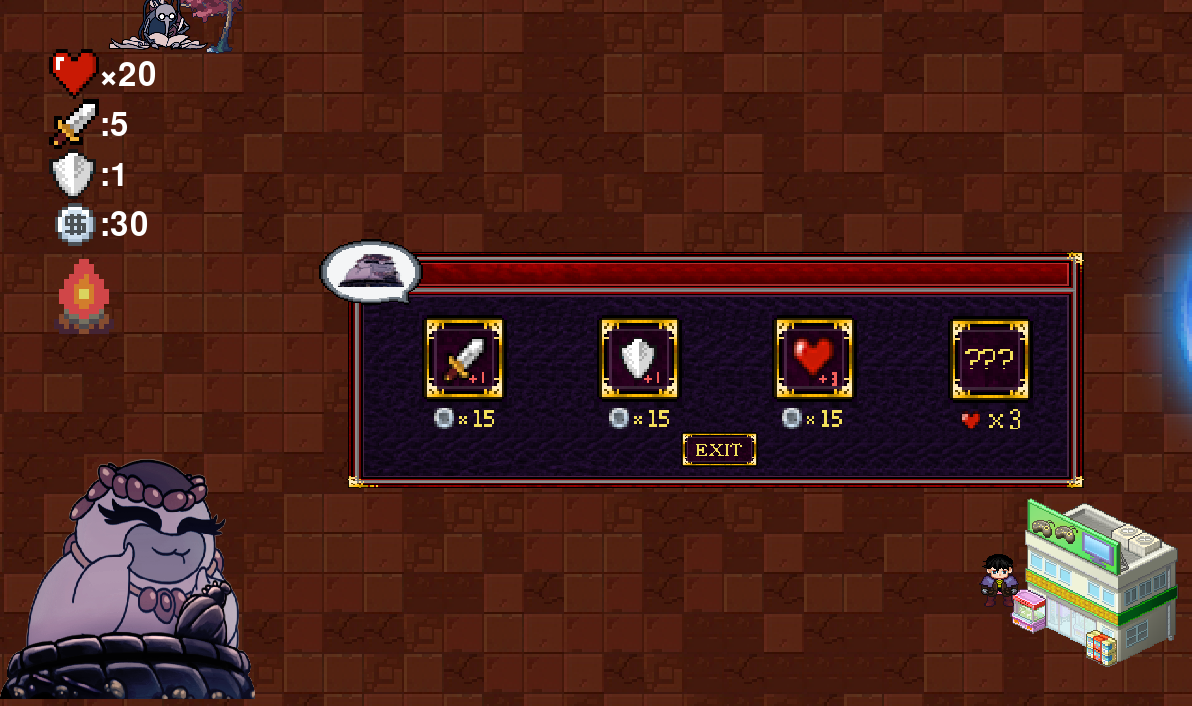
\includegraphics[width=0.75\linewidth]{商店.png}
\caption{\label{fig:商店}商店界面}
\end{figure}

\subsection{火堆}
游戏的城市场景有一个大火堆,诱导玩家探索游戏机制,使玩家发现踩上火堆会持续掉血。野外场景会随机生成小火堆作为障碍物的一种,旨在让玩家每次穿越火堆前往自己想去的地方时付出减少血量资源的代价,这更加强调了控制血量在我们游戏中的作用。

\subsection{属性显示}
玩家的所有属性与资源都会人性化地显示在窗口左上角,以方便玩家进行资源管理。其中,玩家的血量在低于10会显示为一个一个小心心,增加玩家在低血量时的紧迫感,如图\ref{fig:属性显示}。
\begin{figure}[h]
\centering
\subfigure[高血量情况]{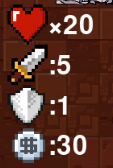
\includegraphics[width=0.2\linewidth]{属性1.png}}
\subfigure[低血量情况]{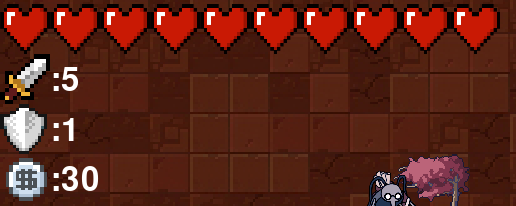
\includegraphics[width=0.6\linewidth]{属性2.png}}
\caption{\label{fig:属性显示}属性显示}
\end{figure}

\subsection{动画}
玩家、怪物、动画树与火堆都有自己独特的动画,使游戏更为生动。玩家往上下左右四个方向行走时动画都不同。
\end{document}